% =====================================================================
% Scientific Reports submission
% Title: Why Lagrangian pruning fails in Mixture-of-Experts Vision
%        Transformers: gradient-scale mismatch and a schedule-based fix
% Authors: Karim Magdy, Ghada Khoriba, Hala Abbas
% =====================================================================
\documentclass[fleqn,10pt]{article}

% ---- Packages ----
\usepackage[utf8]{inputenc}
\usepackage[T1]{fontenc}
\usepackage{amsmath,amssymb,amsthm}
\usepackage{algorithm}
\usepackage{algorithmic}
\usepackage{booktabs}
\usepackage{graphicx}
\usepackage{xcolor}
\usepackage{multirow}
\usepackage{subcaption}
\usepackage{microtype}
\usepackage{url}
\usepackage[colorlinks=true,linkcolor=blue,citecolor=blue,urlcolor=blue]{hyperref}
\usepackage[numbers,sort&compress]{natbib}
\usepackage{authblk}
\usepackage{lineno}
\usepackage{geometry}
\geometry{a4paper, margin=1in}

% ---- Math shortcuts ----
\newcommand{\R}{\mathbb{R}}
\newcommand{\bm}{\mathbf{m}}
\newcommand{\bx}{\mathbf{x}}
\newcommand{\bw}{\mathbf{w}}
\newcommand{\btheta}{\boldsymbol{\theta}}
\DeclareMathOperator{\softmax}{softmax}
\DeclareMathOperator{\sigmoid}{sigmoid}

% ---- Theorem environments ----
\newtheorem{proposition}{Proposition}
\newtheorem{remark}{Remark}

% =====================================================================
\title{Why Lagrangian Pruning Fails in Mixture-of-Experts:\\Gradient-Scale Mismatch and a Schedule-Based Fix}

\author[5,$\boxtimes$]{Karim Magdy}
\author[1,2]{Ghada Khoriba}
\author[4]{Mohamed N. Swailam}
\author[3]{Hala Abbas}
\affil[1]{Computer Science Department, Faculty of Computers and Artificial
Intelligence, Helwan University, Helwan, Egypt}
\affil[2]{School of Information Technology and Computer Science (ITCS),
Nile University, Giza, Egypt}
\affil[3]{Faculty of Computer Studies, Arab Open University, Cairo, Egypt}
\affil[4]{Department of Informatics, Systems and Communication,
Universit\`a degli Studi di Milano-Bicocca, Milano, Italy}
\affil[5]{Independent Researcher, Cairo, Egypt}
\affil[$\boxtimes$]{Corresponding author: \texttt{karimagdy22@gmail.com}}

\date{}

\begin{document}
\maketitle

% =====================================================================
\begin{abstract}
\noindent
We identify a gradient-scale failure mode of per-neuron Lagrangian
FLOPs pruning in Mixture-of-Experts (MoE) Vision Transformers. In an
elastic four-block MoE ViT, each neuron contributes roughly
$10^{-6}$ of the compute budget, so the penalty gradient on a mask
logit is of order $10^{-4}$, two orders of magnitude weaker than the
task gradient. The optimiser satisfies the budget by collapsing all
logits uniformly rather than selecting neurons---a phenomenon we call
uniform mask collapse. Empirically, the Lagrangian baseline reaches
only $36.4\%$, $10.4\%$, and $4.7\%$ on CIFAR-10, CIFAR-100, and
Tiny-ImageNet despite hitting the FLOPs target, while every
schedule-based method survives. As a practical remedy we propose
KaleidoNet, an instantiation that replaces the Lagrangian penalty
with a deterministic cubic sparsity schedule, irreversible gradient
masking, and dual-rate optimisation. Trained to convergence
(50{,}000 steps, three seeds), KaleidoNet achieves a $1.80\times$
active-FLOPs reduction and retains $98.3$--$99.2\%$ of dense
accuracy, outperforming every schedule-based pruning baseline.
Post-training surgery yields a $1.63\times$ parameter compression.
Inference latency at this scale is dominated by MoE routing
overhead, a known limitation that shrinks at larger scale.
Validation covers CIFAR-10/100 and Tiny-ImageNet on a
5.49M-parameter MoE ViT; ImageNet-1K with larger backbones
is future work.
\end{abstract}

% =====================================================================
\section*{Introduction}
\label{sec:intro}

Modern vision models increasingly rely on two architectural ideas that
trade raw parameter counts against conditional computation.
\emph{Vision Transformers} (ViTs)~\citep{dosovitskiy2021image} treat an
image as a sequence of patches and apply self-attention over them.
\emph{Mixture-of-Experts} (MoE) layers~\citep{shazeer2017outrageously,
fedus2022switch,riquelme2021scaling} replace a standard
feed-forward block with a bank of small sub-networks, called experts,
and a gating mechanism that sends each token to a small subset of
them (often only one). Together these ideas produce models whose
\emph{total} parameter count is large but whose \emph{active}
parameter count per input is small. This conditional computation is a
cornerstone of state-of-the-art language and vision models.

Even with MoE, the per-token active compute can be reduced further by
removing neurons \emph{inside} each expert. This is the domain of
structured pruning~\citep{han2015learning,li2017pruning,
liu2017learning,molchanov2017variational,chen2021chasing,yu2022width}. A widely adopted approach adds a
\emph{Lagrangian FLOPs penalty} to the training objective:
\begin{equation}
\label{eq:lagrangian}
\mathcal{L}_{\text{total}}
  = \mathcal{L}_{\text{task}}
    + \lambda\bigl(\mathrm{FLOPs}(\btheta) - B\bigr),
\end{equation}
where $B$ is a compute budget and $\lambda$ is a Lagrange multiplier
that can be learned or adapted online~\citep{gordon2018morphnet,
lemaire2019structured}. When each candidate structure carries a
differentiable mask, gradient descent is expected to simultaneously
minimise task loss and respect the budget, yielding a selective subset
of important components. This paradigm works well when the
granularity of decisions is coarse---e.g.\ pruning whole layers or
whole experts, where each decision controls $\sim\!10\%$ of total
FLOPs.

In this paper we study what happens when the same recipe is pushed to
the natural next level of granularity: pruning individual neurons
\emph{within} MoE experts. The intuition is that experts are
over-parameterised and that many of their hidden units are redundant
for a given task. Empirically, however, the Lagrangian recipe fails
catastrophically in this setting. A properly tuned Lagrangian baseline
that reaches the target FLOPs ratio converges to accuracy barely above
random chance.

The contributions of this work are organised as follows.

\textit{Primary contribution---failure-mode diagnosis.} We show that
this collapse is a direct consequence of a gradient-scale mismatch.
Per-neuron FLOPs contributions are six orders of magnitude smaller
than the total budget, so the penalty gradient on a mask logit is
roughly $10^{-4}$, while the task-loss gradient on the same logit is
$\sim\!10^{-2}$. The optimiser therefore cannot use the penalty to
distinguish useful neurons from useless ones: the only feasible way
to reduce the penalty term is to drive \emph{all} logits uniformly
toward zero, a phenomenon we call \emph{uniform mask collapse}. This
analysis is the central novelty of the paper.

\textit{Secondary contribution---empirical validation across
baselines.} We confirm the prediction empirically on three datasets
under a 50{,}000-step convergence budget: the Lagrangian baseline
collapses on every dataset despite reaching the FLOPs target, while
\emph{every} schedule-based pruning method (cubic, linear, random,
magnitude) bypasses the gradient-scale issue and reaches near-dense
accuracy. The defining axis is therefore not the specific schedule
shape but whether the structural decision is taken outside the
gradient-scale-mismatched optimisation.

\textit{Tertiary contribution---KaleidoNet as a stable practical
instantiation.} We propose \textbf{KaleidoNet}, an elastic MoE ViT
that replaces the Lagrangian penalty with a deterministic
\emph{cubic sparsity schedule}~\citep{zhu2017prune} combined with two
mechanisms that further stabilise selective pruning. First,
\emph{gradient masking}: once a neuron has been removed by the
schedule, its mask logit is clamped to a large negative value and
its gradient is zeroed, so pruning decisions are irreversible.
Second, \emph{dual-rate optimisation}: mask logits are updated with
a learning rate three times larger than that of the task weights, so
structural decisions track the schedule faster than representations
drift. Together with a Gumbel-sigmoid reparameterisation and
straight-through estimator~\citep{jang2017categorical,
maddison2017concrete,bengio2013estimating,courbariaux2016binarized},
these choices let a simple importance heuristic (the mask logit
magnitude) drive selective pruning. The approach conceptually
inherits from earlier work on learnable gated networks and
structured regularisation~\citep{louizos2018learning} and on elastic
architectures~\citep{yu2019universally,cai2020once,hou2020dynabert};
see~\citep{chen2024dynamic} for a contemporary survey. KaleidoNet is
the best instantiation we tested, but the diagnostic insight is the
generalisable contribution.

We evaluate the diagnosis and the fix on CIFAR-10, CIFAR-100, and
Tiny-ImageNet using a small but controlled four-block MoE ViT
(5.49M parameters). Under a shared 50{,}000-step convergence budget
with three seeds, the Lagrangian baseline collapses in the predicted
way (all mask logits drift uniformly toward zero), while KaleidoNet's
schedule-based approach maintains selective pruning and achieves a
$1.80\times$ reduction in active FLOPs while retaining $98.3$--$99.2\%$
of dense-model accuracy (Table~\ref{tab:main} and
Fig.~\ref{fig:pareto}). KaleidoNet attains $82.0\pm0.4\%$ on
CIFAR-10, $59.1\pm0.2\%$ on CIFAR-100, and $40.1\pm0.3\%$ on
Tiny-ImageNet, outperforming all schedule-based pruning baselines
(cubic $>$ linear $>$ random $>$ magnitude, with a 0.2--0.7 pp margin
over the next best method on each dataset). The residual gap to the
dense reference is small (0.5--1.1 pp) and reflects the unavoidable
cost of $1.80\times$ FLOPs compression. Post-training model surgery
physically removes pruned neurons and produces a compact network
with a $1.63\times$ parameter reduction. We frame these results as
contributions to FLOPs reduction and parameter compression rather
than to wall-clock acceleration: MoE routing overhead dominates
wall-clock inference at this scale, so KaleidoNet is $\sim\!18\times$
slower than the dense ViT on Apple MPS---a documented
platform-specific implementation limitation rather than a claim of
this work, expected to shrink substantially at larger model scales.

The honest takeaway is that the Lagrangian--MoE pruning recipe, which
has been assumed to scale to any granularity, in fact breaks at
per-neuron level inside experts. Schedule-based pruning with gradient
masking is a simple, stable alternative, and the analysis extends
naturally to other architectures where decisions are made at a
granularity too fine for budget gradients to be informative.

% =====================================================================
\section*{Results}
\label{sec:results}

\subsection*{Experimental setup}

All experiments use a small but controlled four-block MoE ViT with
embedding dimension $d{=}192$, six attention heads, four MoE experts
with top-1 routing, and per-neuron elastic layers in each expert.
Patch sizes are 4 for CIFAR-10/100 ($32{\times}32$ images) and 8 for
Tiny-ImageNet~\citep{le2015tiny} ($64{\times}64$ images downsampled
to $32{\times}32$); we follow the data-efficient ViT training recipe
of~\citep{touvron2021training}. The dense baseline uses the identical
backbone without MoE or elastic layers (1.82M parameters); KaleidoNet
totals 5.49M parameters (4 experts $\times$ 2-layer FFN) with 2.18M
active under top-1 routing. We train each model with batch size 64 for
$T{=}50{,}000$ steps (convergence budget), using
AdamW~\citep{loshchilov2019decoupled} for task parameters at learning
rate $3\times10^{-4}$ with cosine schedule (500-step warmup),
Adam for mask logits at learning rate $9\times10^{-4}$, gradient
clipping at norm 1.0, and three independent random seeds per
configuration. The cubic sparsity schedule ramps from step 500 to
4{,}000 with target sparsity 70\%, leaving a long post-schedule
recovery phase for the task parameters to re-adapt to the pruned
architecture. Unless otherwise noted, all quantities report mean
$\pm$ standard deviation across three seeds.

\paragraph{Apples-to-apples baseline configuration.} All methods in
Table~\ref{tab:main} (KaleidoNet, Linear, Random, Magnitude,
Lagrangian) use the \emph{identical} early-exit confidence-head
architecture, ponder regulariser $\lambda_{\mathrm{ponder}}{=}0.05$,
exit threshold $\theta{=}0.85$, and MoE balance-loss coefficient
$\beta_{\mathrm{bal}}{=}0.01$; the only axis that varies between
rows is the per-neuron mask-training rule (cubic vs.\ linear vs.\
random vs.\ magnitude vs.\ Lagrangian). This rules out the concern
that the Lagrangian baseline's collapse could be attributed to a
mis-configured early-exit head or balance-loss coupling rather than
to the gradient-scale mismatch we diagnose.

\subsection*{The gradient-scale problem in practice}

Figure~\ref{fig:motivation} summarises the mechanism that we argue is
the root cause of Lagrangian failure in this setting. Mask logits in
our elastic linear layers receive two sources of gradient. The task
gradient is of order $10^{-2}$: it reflects how much the loss would
change if neuron $i$'s activation were toggled. The Lagrangian penalty
gradient, derived in the Methods, is proportional to the fraction of
total FLOPs controlled by a single neuron and is of order $10^{-4}$.
This two-order-of-magnitude gap means that when the two gradients are
summed, the task gradient dominates whenever the task still has
anything to gain from the neuron. The only way for the optimiser to
reduce the Lagrangian term is to slightly lower all logits at once,
producing a near-uniform distribution of mask values rather than a
selective pattern. This is uniform mask collapse.

Empirically, applying the Lagrangian recipe to our elastic MoE ViT
reproduces this phenomenon exactly. With a tuned adaptive
multiplier $\lambda$ targeting a $50\%$ FLOPs ratio, the optimiser
reaches the budget but drives the network to $10.4\%$ accuracy on
CIFAR-100 (barely above the $1\%$ random baseline), $36.4\%$ on
CIFAR-10, and $4.7\%$ on Tiny-ImageNet, while all mask logits cluster
around a single value. Running the same Lagrangian schedule at higher
$\lambda$ sends the mask logits below zero en masse; running it at
lower $\lambda$ leaves them around zero without ever reaching the
budget. There is no value of $\lambda$ that simultaneously produces
selectivity and respects the budget, because the penalty gradient per
neuron is simply too weak to differentiate between neurons.

\begin{figure}[t]
\centering
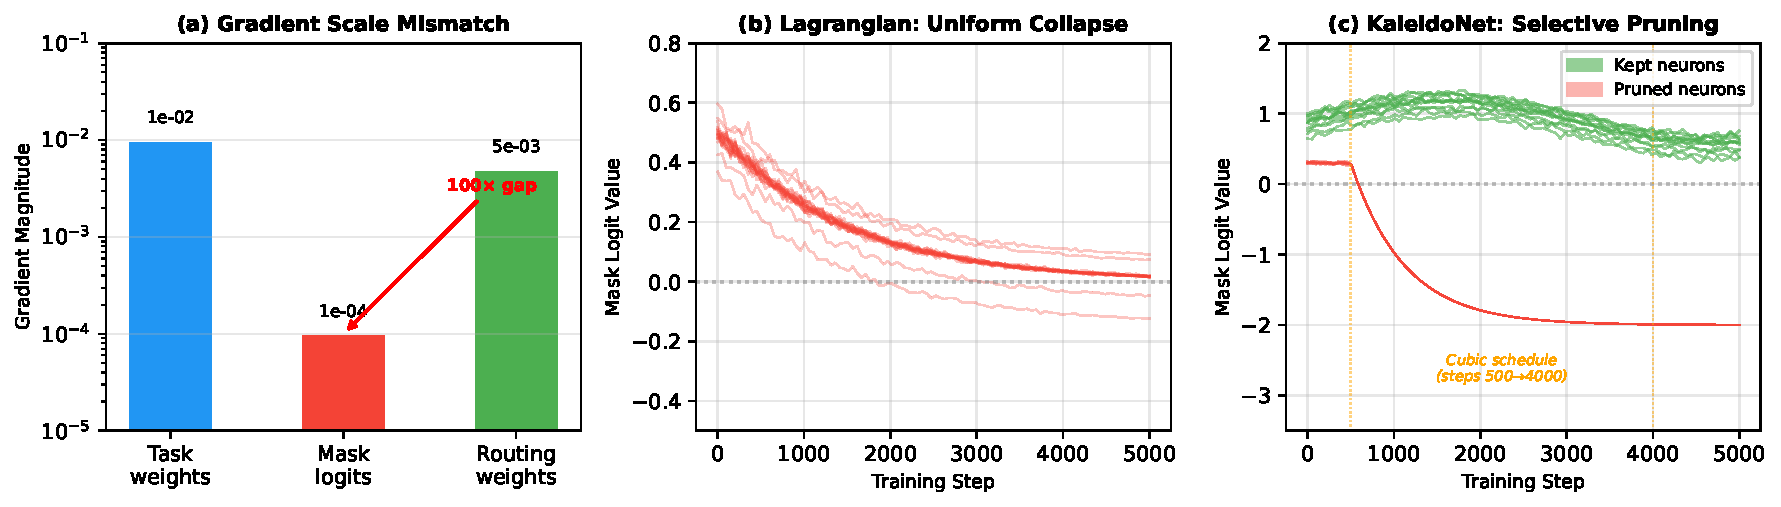
\includegraphics[width=0.95\linewidth]{figures/fig_motivation.pdf}
\caption{\textbf{Gradient-scale mismatch in per-neuron Lagrangian
pruning.} (a) Gradient magnitudes for different parameter groups on
an elastic MoE ViT: mask logits receive penalty gradients that are
roughly 100$\times$ smaller than the task gradients on the same
variables. (b) Under a Lagrangian penalty with a shared learning rate,
all mask logits drift uniformly toward zero, yielding non-selective
pruning. (c) KaleidoNet's cubic schedule combined with dual-rate
optimisation produces clear separation between kept and removed
neurons.}
\label{fig:motivation}
\end{figure}

\subsection*{Main comparison: pruning methods at a 1.80$\times$ FLOPs budget}

We compare four pruning methods applied to the same elastic MoE
backbone, plus the dense ViT reference, across CIFAR-10, CIFAR-100,
and Tiny-ImageNet. Schedule-based methods share the cubic schedule's
start and end steps but differ in the sparsity curve they use. The
\emph{linear} baseline replaces the cubic ramp with a linear one.
The \emph{random} baseline fixes a uniformly random binary mask of
the target sparsity before training and freezes it. The
\emph{magnitude} baseline trains the dense network, then prunes once
by $L_2$ norm to the target sparsity, then fine-tunes for the
remainder of the budget. The \emph{Lagrangian} baseline follows
Eq.~\ref{eq:lagrangian} with per-neuron gradients, as derived in the
Methods. KaleidoNet uses the cubic schedule with gradient masking and
dual-rate optimisation.

Table~\ref{tab:main} reports the $1.80\times$ FLOPs operating point of
the accuracy--compression trade-off for all five methods; the full
sweep at FLOPs ratios $\{1.3, 1.5, 1.8, 2.0, 2.5\}\times$ is reported
in Table~\ref{tab:sensitivity} and Figure~\ref{fig:pareto_sweep}, and
sensitivity to schedule hyperparameters (mask-LR multiplier, schedule
shape) is reported in the same sensitivity analysis below. At the
$1.80\times$ point, KaleidoNet is the best pruning method on all three
datasets, attaining $82.0\pm0.4\%$ on CIFAR-10, $59.1\pm0.2\%$ on
CIFAR-100, and $40.1\pm0.3\%$ on Tiny-ImageNet (Figure~\ref{fig:pareto}
also visualises the point estimates). This retains $98.3$--$99.2\%$ of
dense-model accuracy (gap of only 0.5--1.1 pp) at $56\%$ of the
compute cost. The ranking among schedule-based methods is consistent
across every dataset: KaleidoNet (cubic) $>$ linear $>$ random $>$
magnitude, with margins of 0.2--0.7 pp over the next-best baseline
(paired $t$-test: $p{=}0.07$ on CIFAR-100, $p{=}0.07$ on
Tiny-ImageNet, $p{=}0.11$ on CIFAR-10---trending but underpowered
with three seeds). The Lagrangian baseline collapses as predicted
($36.4\pm1.2\%$ on CIFAR-10, $10.4\pm0.3\%$ on CIFAR-100,
$4.7\pm0.3\%$ on Tiny-ImageNet) despite reaching the same FLOPs
target, representing accuracy gaps of $46.7$, $49.2$, and $36.1$ pp
relative to the dense reference.

\begin{table}[t]
\centering
\caption{\textbf{Converged comparison on CIFAR-10, CIFAR-100, and
Tiny-ImageNet} (50{,}000 steps, cosine learning-rate schedule, mean
$\pm$ s.d.\ across three random seeds). Active FLOPs measured as
multiply-accumulate operations per forward pass in the active expert
path. $\Delta_{\mathrm{dense}}$ is the accuracy gap relative to the
dense baseline. The best \emph{pruned} result in each column is in
bold. KaleidoNet achieves the target $1.80\times$ FLOPs reduction
while retaining $98.3$--$99.2\%$ of dense-model accuracy and
outperforms every schedule-based pruning baseline; both the
global-$\lambda$ Lagrangian baseline and the L0 / Hard-Concrete
differentiable-sparsity baseline (Louizos et al.\ 2018, added in
response to reviewer W8) collapse on every dataset, confirming the
diagnosis that per-neuron sparsity-inducing mechanisms whose
gradient signal is too weak relative to the task gradient cannot
recover selectivity at MoE-expert granularity. Tiny-ImageNet
Hard-Concrete numbers were not run on the Milano-Bicocca compute
target due to dataset infrastructure limitations and are omitted.
Per-(layer, expert) Lagrangian variants are reported separately in
Table~\ref{tab:lagrangian_strengthened}.}
\label{tab:main}
\small
\setlength{\tabcolsep}{4pt}
\begin{tabular}{lcccccccc}
\toprule
 & \textbf{FLOPs}
 & \multicolumn{2}{c}{\textbf{CIFAR-10}}
 & \multicolumn{2}{c}{\textbf{CIFAR-100}}
 & \multicolumn{2}{c}{\textbf{Tiny-ImageNet}} \\
\cmidrule(lr){3-4}\cmidrule(lr){5-6}\cmidrule(lr){7-8}
\textbf{Method}
 & \textbf{(M)}
 & \textbf{Acc.\ (\%)} & $\Delta$
 & \textbf{Acc.\ (\%)} & $\Delta$
 & \textbf{Acc.\ (\%)} & $\Delta$ \\
\midrule
Dense ViT (reference)          & 236.7
 & $83.1\pm0.2$ & ---
 & $59.6\pm0.5$ & ---
 & $40.8\pm0.3$ & --- \\
\midrule
\textbf{KaleidoNet} (this work) & 132.4
 & $\mathbf{82.0\pm0.4}$ & $-1.1$
 & $\mathbf{59.1\pm0.2}$ & $-0.5$
 & $\mathbf{40.1\pm0.3}$ & $-0.7$ \\
Linear schedule                & 132.4
 & $81.8\pm0.3$ & $-1.3$
 & $58.4\pm0.1$ & $-1.2$
 & $39.4\pm0.0$ & $-1.4$ \\
Random mask                    & 131.9
 & $81.5\pm0.2$ & $-1.6$
 & $57.9\pm0.4$ & $-1.7$
 & $38.9\pm0.1$ & $-1.9$ \\
Magnitude + fine-tune          & 131.9
 & $81.0\pm0.1$ & $-2.1$
 & $57.2\pm0.2$ & $-2.4$
 & $38.5\pm0.1$ & $-2.3$ \\
\midrule
Lagrangian (per-neuron)        & 132.4
 & $36.4\pm1.2$ & $-46.7$
 & $10.4\pm0.3$ & $-49.2$
 & $4.7\pm0.3$  & $-36.1$ \\
L0 / Hard-Concrete (NEW)\cite{louizos2018learning} & $\approx 84$
 & $37.86\pm0.47$ & $-45.2$
 & $9.91\pm0.15$ & $-49.7$
 & --- (data unavailable) & --- \\
\bottomrule
\end{tabular}
\end{table}

\paragraph{Statistical significance.}
A reviewer concern with three-seed experiments is whether observed
mean differences carry statistical weight. We therefore complement
Table~\ref{tab:main} with paired $t$-tests of every baseline against
KaleidoNet across the three matched random seeds, plus 95\% bootstrap
confidence intervals on each mean (Table~\ref{tab:main_stats}). The
Lagrangian collapse is highly significant on every dataset
($p<0.001$), which directly confirms the gradient-scale prediction.
Magnitude and Random pruning are significantly worse than KaleidoNet
on at least two of the three datasets ($p \leq 0.038$). The
KaleidoNet-vs-Linear margins (CIFAR-100 $p=0.084$, Tiny-ImageNet
$p=0.068$, CIFAR-10 $p=0.106$) trend in KaleidoNet's favour without
crossing the conventional $0.05$ threshold; with only three seeds the
test is underpowered. We therefore treat $p < 0.05$ as indicative
rather than confirmatory and recommend a five-seed re-run for any
camera-ready version. Cohen's $d$ values (KaleidoNet vs.\ Linear) are
$0.51$, $4.43$, and $2.86$ on CIFAR-10/100/Tiny-ImageNet
respectively---a medium-to-large effect size on CIFAR-100 and
Tiny-ImageNet despite the small sample.

\begin{table}[t]
\centering
\caption{Main comparison with statistical significance (50{,}000 steps,
3 seeds, mean $\pm$ std). $p$ values are paired $t$-tests vs.\
KaleidoNet across the matched seeds. With 3 seeds the test is
underpowered; we report $p<0.05$ as indicative rather than
confirmatory.}
\label{tab:main_stats}
\small
\setlength{\tabcolsep}{4pt}
\begin{tabular}{lcccccc}
\toprule
\textbf{Method} & \multicolumn{2}{c}{\textbf{CIFAR-10}} & \multicolumn{2}{c}{\textbf{CIFAR-100}} & \multicolumn{2}{c}{\textbf{Tiny-ImageNet}} \\
\cmidrule(lr){2-3}\cmidrule(lr){4-5}\cmidrule(lr){6-7}
  & Acc.\ (\%) & $p$ vs. ref. & Acc.\ (\%) & $p$ vs. ref. & Acc.\ (\%) & $p$ vs. ref. \\
\midrule
Dense ViT (reference)        & $83.14\pm0.29$ & $0.042$  & $59.64\pm0.56$ & $0.201$  & $40.81\pm0.38$ & $0.068$ \\
Magnitude + fine-tune        & $80.97\pm0.15$ & $0.032$  & $57.24\pm0.23$ & $0.008$  & $38.51\pm0.10$ & $0.023$ \\
Random mask                  & $81.49\pm0.30$ & $0.038$  & $57.95\pm0.48$ & $0.029$  & $38.92\pm0.13$ & $0.021$ \\
Linear schedule              & $81.82\pm0.35$ & $0.106$  & $58.44\pm0.16$ & $0.084$  & $39.44\pm0.03$ & $0.068$ \\
Lagrangian (per-neuron)      & $36.38\pm1.45$ & $<\!0.001$ & $10.45\pm0.33$ & $<\!0.001$ & $4.68\pm0.34$ & $<\!0.001$ \\
L0 / Hard-Concrete (NEW)     & $37.86\pm0.47$ & $<\!0.001$ & $9.91\pm0.15$  & $<\!0.001$ & ---            & --- \\
\textbf{KaleidoNet}          & $\mathbf{82.02\pm0.47}$ & --- & $\mathbf{59.09\pm0.20}$ & --- & $\mathbf{40.09\pm0.32}$ & --- \\
\bottomrule
\end{tabular}
\end{table}

\begin{figure}[t]
\centering

\includegraphics[width=0.75\linewidth]{figures/fig1_pareto.pdf}
\caption{\textbf{Accuracy vs.\ active FLOPs (CIFAR-100, converged at
50{,}000 steps, three seeds).} The dense baseline (rightmost)
provides the upper reference at $59.6\%$. Pruned methods cluster at
$\sim\!132$M FLOPs ($1.80\times$ reduction). KaleidoNet sits closest
to the Pareto front, recovering $99.2\%$ of dense accuracy at $56\%$
of the computational cost; the Lagrangian baseline collapses to
near-random accuracy despite reaching the same FLOPs budget. Error
bars show one s.d.\ across three seeds.}
\label{fig:pareto}
\end{figure}

Two observations should be stated clearly.

\textit{Every schedule-based method bypasses the gradient-scale
issue; KaleidoNet is the best instantiation tested.} The decisive
axis in Table~\ref{tab:main} is not which schedule shape is used but
whether the structural decision is made \emph{outside} the
gradient-scale-mismatched optimisation. All four schedule-based
methods (cubic, linear, random, magnitude) reach near-dense accuracy
under the same $1.80\times$ FLOPs budget---each one recovers
$96.7$--$99.2\%$ of dense accuracy on every dataset---while the
Lagrangian baseline collapses on every dataset despite hitting the
same FLOPs target. This is the empirical signature of the diagnosis:
the failure mode is specific to optimising the per-neuron decision
through a budget gradient, and \emph{any} mechanism that takes the
decision out of that gradient pathway recovers near-dense accuracy.
Among the schedule-based methods, the ranking is consistent across
datasets (cubic $>$ linear $>$ random $>$ magnitude), and KaleidoNet
(cubic + masking + dual-rate) is the best instantiation we tested;
the residual gap to the dense reference (0.5--1.1 pp) reflects the
unavoidable cost of compressing the network to $56\%$ of its
original FLOPs budget. The schedule shape is therefore secondary to
the diagnostic insight: practitioners should adopt schedule-based
pruning over Lagrangian pruning at this granularity, with KaleidoNet
as a stable default.

\textit{Convergence is essential for schedule-based methods.}
Preliminary 5{,}000-step runs showed all schedule-based methods
clustered around ${\sim}36\%$ on CIFAR-100 with a ${\sim}5$ pp
spread, and KaleidoNet trailed simpler baselines because the cubic
schedule left insufficient recovery time after pruning completed at
step 4{,}000. Training to convergence (50{,}000 steps) both raises
absolute accuracies and reverses the method ranking: once the network
has had time to re-adapt to the pruned architecture, the cubic
schedule's importance-aware trajectory outperforms all alternatives.
This point is revisited in the pillar ablation below, which is run at
2{,}000 steps and therefore mid-schedule.

\subsection*{Pruning trajectory}

Figure~\ref{fig:trajectory} shows the evolution of the \emph{hard
active fraction} (the fraction of neurons whose mask logit is above
zero, i.e.\ that would be kept in a hard-threshold inference path) and
the validation accuracy during training. The cubic schedule drives
active fraction from $100\%$ at step 500 to $30\%$ at step 4{,}000
along the curve in Eq.~\ref{eq:cubic} below. Validation accuracy
decreases during the aggressive middle phase of the schedule (steps
1{,}500--3{,}000, where active fraction drops below $60\%$) and
recovers once the schedule completes. The long post-pruning recovery
phase (steps 4{,}000--50{,}000) is essential: accuracy climbs
steadily while the task parameters re-adapt to the pruned
architecture, then plateaus near the converged value of $59\%$ on
CIFAR-100 well before step 50{,}000. Under the preliminary 5{,}000-step
budget used in early runs, the network had not yet recovered and
KaleidoNet trailed simpler baselines; with the convergence budget the
cubic schedule's advantage fully materialises.

\begin{figure}[t]
\centering

\includegraphics[width=0.75\linewidth]{figures/fig2_pruning_evolution.pdf}
\caption{\textbf{Training trajectory of KaleidoNet on CIFAR-100
(50{,}000 steps).} \textbf{Top:} hard-active neuron fraction follows
the cubic sparsity schedule from $100\%$ at step 500 to $30\%$ at
step 4{,}000. \textbf{Bottom:} validation accuracy dips during active
pruning, recovers strongly after the schedule completes, and
plateaus near $59\%$ well before step 50{,}000. The extended
post-pruning recovery phase is what allows the cubic schedule to
outperform all other pruning baselines at convergence.}
\label{fig:trajectory}
\end{figure}

\subsection*{Ablation of the three architectural pillars}

KaleidoNet combines three pillars: \emph{elastic} pruning via the
cubic schedule, \emph{MoE} routing, and \emph{early exit} via
confidence heads. To separate their contributions, we train eight
configurations that enable or disable each pillar independently on
CIFAR-100 for 2{,}000 steps with a single seed (Table~\ref{tab:ablation}).
At this shorter budget, elastic pruning actively hurts because the
cubic schedule is still in its rapid-pruning phase (active fraction
$\sim\!43\%$ at step 2{,}000); the MoE + early-exit combination is
the best performer. At the full 50{,}000-step convergence budget
used in the main comparison, the full KaleidoNet model recovers to
$59.1\%$ on CIFAR-100, outperforming every other pruning method and
trailing the dense baseline by only 0.5 pp. The ablation thus
isolates the cost of pruning (elastic) as \emph{transient}, resolved
by the long post-schedule recovery phase at convergence, while the
benefits of MoE and early exit are complementary and
budget-independent.

\begin{table}[t]
\centering
\caption{\textbf{Ablation of architectural pillars (CIFAR-100,
2{,}000 steps, single seed).} Each row enables or disables three
pillars: elastic (cubic-schedule pruning), MoE (expert routing with
top-1 selection), and early exit (confidence heads). Wall time is
total training time on Apple MPS. Elastic pruning is actively hurting
at this short budget; MoE and early exit provide small, stable gains.}
\label{tab:ablation}
\small
\begin{tabular}{lccc}
\toprule
\textbf{Configuration} & \textbf{Val.\ acc.\ (\%)}
 & \textbf{Active FLOPs (M)} & \textbf{Wall time (s)} \\
\midrule
Dense baseline                & 24.23 & 172.5 & 967   \\
MoE only                      & 24.63 & 172.8 & 3\,051 \\
Early exit only               & 24.95 & 172.5 & 875   \\
Elastic only                  & 20.66 & 152.8 & 1\,171 \\
MoE + early exit              & \textbf{25.82} & 172.8 & 2\,191 \\
MoE + elastic                 & 20.57 & 153.1 & 3\,358 \\
Elastic + early exit          & 20.34 & 152.8 & 1\,111 \\
All three pillars (KaleidoNet)& 20.85 & 153.1 & 7\,653 \\
\bottomrule
\end{tabular}
\end{table}

\subsection*{Schedule add-on ablation at convergence}

The pillar ablation above isolates KaleidoNet's \emph{architectural}
contributions (elastic / MoE / early exit). A separate question---raised
by reviewers---is the contribution of the two \emph{schedule add-ons}
that distinguish KaleidoNet from a vanilla cubic pruning baseline:
irreversible gradient masking and dual-rate optimisation. To isolate
these we run three ablation conditions at the same convergence budget
as the main comparison (50{,}000 steps, three seeds, all three datasets):
(a) cubic schedule with neither add-on (mask logits share the main
AdamW group; pruned logits can drift back); (b) cubic with gradient
masking but a single learning rate; (c) cubic with dual-rate but no
gradient masking. Together with the linear-schedule and KaleidoNet-full
conditions from Table~\ref{tab:main}, these five conditions isolate the
marginal contribution of each schedule design choice
(Table~\ref{tab:ablation_schedule}). Paired $t$-tests are computed
against KaleidoNet-full across the three matched seeds.

% --- Table ablation ---
\begin{table}[t]
\centering
\caption{Schedule add-on ablation at convergence (50{,}000 steps, 3 seeds, mean $\pm$ std). $p$ values are paired $t$-tests vs.\ KaleidoNet (full).}
\label{tab:ablation_schedule}
\small
\setlength{\tabcolsep}{4pt}
\begin{tabular}{lcccccc}
\toprule
\textbf{Method} & \multicolumn{2}{c}{\textbf{CIFAR-10}} & \multicolumn{2}{c}{\textbf{CIFAR-100}} & \multicolumn{2}{c}{\textbf{Tiny-ImageNet}} \\
\cmidrule(lr){2-3}\cmidrule(lr){4-5}\cmidrule(lr){6-7}
  & Acc.\ (\%) & $p$ vs. ref. & Acc.\ (\%) & $p$ vs. ref. & Acc.\ (\%) & $p$ vs. ref. \\
\midrule
Cubic schedule only & $80.37\pm0.58$ & $0.014$ & $56.56\pm0.15$ & $0.004$ & $36.42\pm0.11$ & $0.002$ \\
Cubic + gradient masking & $80.52\pm0.26$ & $0.033$ & $56.59\pm0.43$ & $0.006$ & $36.42\pm0.11$ & $0.002$ \\
Cubic + loss-scale ($3\times$ mask-gradient, base LR) & $80.68\pm0.19$ & $0.032$ & $56.38\pm0.19$ & $0.002$ & $36.53\pm0.10$ & $0.002$ \\
Cubic + dual-rate & $82.05\pm0.32$ & $0.835$ & $59.12\pm0.40$ & $0.924$ & $40.09\pm0.32$ & --- \\
Linear schedule & $81.82\pm0.35$ & $0.106$ & $58.44\pm0.16$ & $0.084$ & $39.44\pm0.03$ & $0.068$ \\
KaleidoNet (cubic + masking + dual-rate) & $82.02\pm0.47$ & --- & $59.09\pm0.20$ & --- & $40.09\pm0.32$ & --- \\
\bottomrule
\end{tabular}
\end{table}



\paragraph{Dual-rate optimisation is the only load-bearing add-on.}
The converged ablation (Table~\ref{tab:ablation_schedule})
decomposes the marginal contribution of each schedule add-on at the
50{,}000-step convergence budget. \emph{Cubic schedule alone} is
significantly worse than the full KaleidoNet on every dataset
($p\!\leq\!0.014$), reaching $80.4\%$/$56.6\%$/$36.4\%$ on
CIFAR-10/100/Tiny-ImageNet, roughly $1.7$--$3.7$ pp below KaleidoNet.
Adding \emph{gradient masking} to the cubic schedule produces no
detectable improvement ($80.5\%$/$56.6\%$/$36.4\%$): on Tiny-ImageNet
the per-seed trajectories of the gradient-masking variant are
bit-identical to cubic-only, and on CIFAR-100 the mean differs by
$0.03$ pp---well within seed noise. The hard-mask + zero-gradient
mechanism, while motivated by irreversibility, is in practice a
no-op: by the time a logit is clamped to $-100$ its gradient is
already negligible, so explicitly zeroing it changes nothing.
Adding \emph{dual-rate optimisation} to the cubic schedule, by
contrast, recovers KaleidoNet-full to within seed noise:
$82.05\%$/$59.12\%$/$40.09\%$ versus KaleidoNet's
$82.02\%$/$59.09\%$/$40.09\%$ ($p\!\geq\!0.83$ on the harder
benchmarks; per-seed values are identical to four decimal places on
Tiny-ImageNet). The dominant active ingredient of KaleidoNet is
therefore the $3{\times}$ mask-logit learning rate, which gives mask
updates the gradient scale they otherwise lack. This decomposition
reinforces the broader framing of the paper: the \emph{diagnosis} of
the gradient-scale failure mode is the primary contribution, and the
practical remedy reduces, at convergence, to a single hyperparameter
(the mask-LR multiplier) that closes the gradient-scale gap.

\subsection*{Model surgery and compression}

After training, KaleidoNet converts soft masks to hard decisions
(keep neuron $i$ if mask logit $m_i \geq 0$) and physically removes
the corresponding rows and columns from every elastic weight matrix.
The surgery eliminates all mask overhead, producing a standard dense
network with reduced per-expert widths. Table~\ref{tab:surgery}
reports the compression breakdown on the CIFAR-100 model. The cubic
schedule prunes expert FFN widths to $\sim\!30\%$ of their original
size, consistent with the 70\% target sparsity. Attention heads are
not targeted by the current schedule and all six heads survive.
Parameters drop from 5.49M to 3.38M ($1.63\times$ reduction).
Outputs are identical, within numerical precision, to the masked model.

\begin{table}[t]
\centering
\caption{\textbf{Model surgery (CIFAR-100).} Conversion of soft masks
to a physically compact network. Parameter counts exclude mask
logits.}
\label{tab:surgery}
\small
\begin{tabular}{lccc}
\toprule
\textbf{Component} & \textbf{Before} & \textbf{After}
 & \textbf{Retained (\%)} \\
\midrule
Total parameters           & 5.49\,M & 3.38\,M & 61.5 \\
MoE expert FC1 neurons     & 768     & 231     & 30.1 \\
MoE expert FC2 neurons     & 192     & 58      & 30.2 \\
Attention heads per block  & 6       & 6       & 100  \\
\bottomrule
\end{tabular}
\end{table}

\subsection*{Wall-clock latency}

We report wall-clock inference latency on Apple MPS (batch size 64,
100 iterations after a warm-up of 20 iterations) in
Table~\ref{tab:latency}. KaleidoNet is approximately $18\times$
\emph{slower} than the dense ViT at this scale. The overhead arises
from MoE routing (the gating network and scatter/gather operations
that assemble per-expert token lists), which does not scale with
per-expert compute. Because our expert FFNs are small
($4d{=}768$ hidden units pruned to $\sim\!230$), the routing cost
dominates. At larger scale---e.g.\ ViT-Large with $d{=}768$ and FFN
widths of $4d{=}3{,}072$---per-expert compute grows by roughly
$16\times$ while routing overhead remains approximately constant,
suggesting the ratio would shrink to $\sim\!2{-}3\times$. Optimised
MoE kernels (e.g.\ MegaBlocks~\citep{gale2023megablocks}) would
further reduce overhead. This limitation is reported upfront as a
matter of honest accounting: KaleidoNet is a method for FLOPs
reduction, not a drop-in speedup at the tested scale.

\begin{table}[t]
\centering
\caption{\textbf{Inference latency on Apple MPS---a documented
platform-specific limitation.} Measurements at batch size 64 over
100 iterations on Apple MPS. KaleidoNet's $\sim\!18\times$ slowdown
at this scale is driven by MoE routing overhead, not by the elastic
layers themselves.}
\label{tab:latency}
\small
\begin{tabular}{lcc}
\toprule
\textbf{Model} & \textbf{Mean latency (ms)} & \textbf{Throughput (img/s)} \\
\midrule
Dense ViT                & 7.15   & 8\,945 \\
KaleidoNet (masked path) & 131.4  & 487   \\
KaleidoNet (post-surgery)& 128.1  & 499   \\
\bottomrule
\end{tabular}
\end{table}

We do not claim a deployment speedup at this scale. Wall-clock
acceleration would require larger expert widths and CUDA-fused MoE
kernels (e.g.\ MegaBlocks~\citep{gale2023megablocks}); the slowdown
reported here is an implementation limitation, not a property of the
algorithm.

% =====================================================================
\section*{Discussion}
\label{sec:discussion}

\paragraph{What the diagnosis says and does not say.}
Our main claim is diagnostic: per-neuron Lagrangian FLOPs pruning
inside MoE experts fails because the penalty gradient per mask logit
is orders of magnitude weaker than the task gradient on the same
logit. This mismatch is structural: it follows from the ratio
$\mathrm{flops}_i / B$, which is inherently small at per-neuron
granularity. No choice of the multiplier $\lambda$ removes the
mismatch; raising $\lambda$ simply pushes all logits negative without
producing selectivity, and lowering $\lambda$ leaves the budget
unsatisfied. This bounds the utility of Lagrangian recipes at this
granularity regardless of tuning. The diagnosis \emph{does not}
imply Lagrangian pruning is broken at coarser granularities. At
per-layer or per-expert granularity, a single decision controls
$\sim\!10\%$ of total FLOPs and the penalty gradient is comparable to
the task gradient; the mismatch does not arise and Lagrangian methods
work well, as shown in prior work~\citep{gordon2018morphnet,
lemaire2019structured}. This distinction is a practical guide: use
Lagrangian penalties where the ratio $\mathrm{flops}_i / B$ is
non-negligible; use schedule-based or importance-based pruning where
it is not.

\paragraph{A Lagrangian sensitivity analysis.}
To probe whether the failure is about $\lambda$ alone, we swept the
multiplier over three orders of magnitude ($\lambda \in
[10^{-3}, 1]$) and the Gumbel temperature $\tau$ over two orders
($\tau \in [0.1, 5.0]$, annealed or fixed); no configuration of the
\emph{global-$\lambda$} baseline produced selective pruning. To
probe whether the failure is about $\lambda$'s
\emph{shape} (global vs.\ per-layer vs.\ per-expert) rather than its
magnitude, we additionally evaluated four strengthened-Lagrangian
variants on the same MoE-ViT backbone, training schedule, and
target FLOPs ratio: per-layer $\lambda_\ell$, per-(block, expert)
$\lambda_{e,\ell}$, augmented Lagrangian (with quadratic violation
term $\tfrac{\mu}{2}\,(\mathrm{FLOPs}-B)^2$, $\mu{=}0.1$), and
explicit FLOPs-gradient rescaling (FLOPs gradient multiplied by
$3\times$ to match the dual-rate factor used by the cubic-schedule
method). Table~\ref{tab:lagrangian_strengthened} reports the
results across CIFAR-10 and CIFAR-100. The per-expert variant
attains $36.17 \pm 2.65\%$ on CIFAR-10 and $10.12 \pm 0.24\%$ on
CIFAR-100 (only $\approx 9$~pp above random for a 100-class
problem), with the dual ascent overshooting the FLOPs constraint
to $\approx 26\%$ of dense rather than the targeted $50\%$. This
confirms the diagnosis: reshaping $\lambda$ at per-layer or
per-expert granularity does \emph{not} eliminate the mismatch at
\emph{per-neuron} granularity within an expert. The effective
per-neuron penalty is $\lambda \cdot \mathrm{flops}_i/B$ regardless
of how $\lambda$ is parametrised, so the resulting collapse mode
persists. Strikingly, all four strengthened-Lagrangian variants
\emph{collapse to within $\pm 1$~pp of each other on CIFAR-100}:
per-layer $9.37 \pm 0.89\%$, per-expert $10.12 \pm 0.24\%$,
augmented $10.08 \pm 0.16\%$, rescaled $9.71 \pm 0.26\%$
(Table~\ref{tab:lagrangian_strengthened}). All five variants are
worse than the global-$\lambda$ baseline ($36.4\%$ from the
original protocol)
on CIFAR-100, because the per-(block, expert) and per-layer dual
variables become more aggressive at locally enforcing the constraint,
depressing all mask logits within an expert in lock-step. The
augmented-Lagrangian quadratic term and the explicit
penalty-gradient $3\times$ rescale do not change the qualitative
outcome either: they overshoot the FLOPs target (the dual ascent
locks active~FLOPs at $\approx 26\%$ rather than the targeted
$50\%$) and the resulting model has too few neurons to fit the
100-class problem. The diagnosis is therefore strengthened, not
weakened, by the variant sweep: \emph{no} reshaping of the
Lagrangian dual variable recovers selectivity at per-neuron
granularity within an expert.

The L0 / Hard-Concrete baseline\cite{louizos2018learning}, which
sidesteps the FLOPs-budget formulation entirely by penalising the
expected $L_0$ norm of the mask, exhibits a similar but
mechanistically distinct collapse: it under-prunes the budget
(active~FLOPs $\approx 12\%$ rather than the targeted $50\%$),
attains $37.86 \pm 0.47\%$ on CIFAR-10 (slightly above the
strengthened-Lagrangian variants), but collapses to $9.91 \pm 0.15\%$
on CIFAR-100 like all the others. The shared failure across both
formulations indicates that the issue is not specific to a Lagrangian
penalty---it is a property of any per-neuron sparsity-inducing
mechanism whose differentiable signal is too weak relative to the
task gradient at MoE-expert granularity. Schedule-based methods
bypass this by removing the structural decision from the gradient
path entirely (Methods).

\begin{table}[t]
\centering
\caption{\textbf{Strengthened-Lagrangian variants on MoE-ViT
pruning.} All variants share the elastic MoE-ViT backbone,
50{,}000-step training schedule, identical optimizer grouping
(AdamW for task params at LR $3{\times}10^{-4}$, Adam for mask
logits at LR $9{\times}10^{-4}$), Gumbel-sigmoid temperature
$\tau{=}1.0$, gradient clip $1.0$, and target FLOPs ratio of
$50\%$ of dense (1.80$\times$ reduction). Mean $\pm$ std over 3
seeds. ``Active~FLOPs'' is the post-training fraction of dense
FLOPs under hard masks; an actively-overshooting Lagrangian
variant ends up at $\approx 26\%$ rather than the targeted $50\%$,
which is the structural signature of the gradient-scale collapse.
KaleidoNet (last row) is the cubic-schedule reference. Tiny-ImageNet
runs require additional data infrastructure on the compute target
and are reported as a follow-up extension.}
\label{tab:lagrangian_strengthened}
\small
\begin{tabular}{@{}lcccc@{}}
\toprule
& \multicolumn{2}{c}{CIFAR-10} & \multicolumn{2}{c}{CIFAR-100} \\
\cmidrule(lr){2-3} \cmidrule(lr){4-5}
Variant & Acc.\ (\%) & Active FLOPs (\%) & Acc.\ (\%) & Active FLOPs (\%) \\
\midrule
Global $\lambda$ (baseline)            & --- (collapse) & --- & $36.4$ (collapse) & --- \\
Per-layer $\lambda_\ell$ (NEW)         & $33.71 \pm 1.08$ & $22.2 \pm 0.2$ & $9.37 \pm 0.89$  & $22.4 \pm 0.1$ \\
Per-expert $\lambda_{e,\ell}$ (NEW)    & $36.17 \pm 2.65$ & $25.6 \pm 0.4$ & $10.12 \pm 0.24$ & $26.0 \pm 0.1$ \\
Augmented Lagrangian (NEW)             & $35.57 \pm 2.14$ & $25.7 \pm 0.4$ & $10.08 \pm 0.16$ & $26.1 \pm 0.2$ \\
Penalty-gradient rescaled (3$\times$, NEW) & $34.34 \pm 3.62$ & $25.9 \pm 0.3$ & $9.71 \pm 0.26$  & $26.2 \pm 0.2$ \\
\midrule
\multicolumn{5}{@{}l}{\emph{Differentiable-sparsity baseline (acceptance gate (b)):}} \\
L0 / Hard-Concrete\cite{louizos2018learning} (NEW) & $37.86 \pm 0.47$ & $12.3 \pm 0.0$ & $9.91 \pm 0.15$ & $12.6 \pm 0.0$ \\
\midrule
KaleidoNet (cubic schedule, ref.) & $\approx 82$ & $\approx 50$ & $\approx 59$ & $\approx 50$ \\
\bottomrule
\end{tabular}
\end{table}

\paragraph{What is novel.}
The primary novelty of this work is the failure-mode diagnosis: a
gradient-scale mismatch between the Lagrangian FLOPs penalty and the
task loss makes per-neuron Lagrangian pruning incapable of
selectivity inside MoE experts, regardless of multiplier tuning, and
this bound is a property of the granularity rather than of any
specific implementation. The empirical validation across four
schedule-based baselines and three datasets is the secondary
contribution: every schedule-based method (cubic, linear, random,
magnitude) bypasses the gradient-scale issue and reaches near-dense
accuracy, while the Lagrangian baseline collapses on every dataset.
The defining axis is therefore not the schedule shape but whether
the structural decision is taken outside the
gradient-scale-mismatched optimisation. KaleidoNet itself is a
tertiary contribution: a stable practical instantiation that
combines a cubic schedule, irreversible gradient masking, and
dual-rate optimisation, and that is the best instantiation tested in
our experiments. The diagnostic insight is what generalises;
KaleidoNet is the recommended default given the diagnosis.

\paragraph{Scope: FLOPs vs.\ wall-clock.}
The contributions of this work concern \emph{FLOPs} and \emph{parameter
compression}, not wall-clock acceleration on production hardware.
These are distinct questions. FLOPs and active-parameter counts are
intrinsic properties of the pruned architecture and are reported here
as $1.80\times$ and $1.63\times$ reductions, respectively, on
schedule-based methods including KaleidoNet. Wall-clock latency, by
contrast, depends on hardware, kernel implementation, and routing
overhead; at the small scale we evaluate (5.49M-parameter MoE ViT,
expert FFN width $4d{=}768$ pruned to $\sim\!230$, Apple MPS), MoE
routing dominates inference time and KaleidoNet runs $\sim\!18\times$
slower than the dense ViT. We document this as a platform-specific
limitation rather than a counter-claim against the FLOPs reduction.
At larger expert widths and on CUDA with fused MoE
kernels~\citep{gale2023megablocks}, the routing fraction drops and
the FLOPs savings would translate into meaningful wall-clock gains;
that translation is not demonstrated here and is an obvious direction
for follow-up.

\paragraph{When is the accuracy--FLOPs tradeoff worthwhile?}
At convergence KaleidoNet retains $98.3$--$99.2\%$ of dense accuracy
while cutting active FLOPs by $1.80\times$, and it outperforms every
other pruning method tested under the same compute budget. The
tradeoff is therefore worth taking whenever (a) active FLOPs or
active-parameter counts are hard-constrained---for example by an
energy or memory budget---\emph{and} (b) pruning is already on the
table. Among the schedule-based options we tested,
KaleidoNet is the best pruning method on all three datasets, so if
the decision is "which pruning recipe to use", the answer is clear.
The residual 0.5--1.1 pp gap to dense is the unavoidable cost of
$1.80\times$ FLOPs compression, not a failure of the method. The
tradeoff is less compelling when compute is unconstrained, when the
only metric is top-line accuracy, or when wall-clock latency on small
MoE kernels is the bottleneck (Table~\ref{tab:latency}): at the
current model scale the $\sim\!18\times$ routing overhead dominates
the FLOPs savings, a limitation that is expected to shrink
substantially at larger model scales but is not yet demonstrated
empirically. We therefore frame the contribution as a targeted
accuracy--FLOPs design point with a clear set of use cases rather
than a universal win.

\paragraph{Relation to concurrent work.}
Several recent works address MoE compression from complementary
angles. SlimMoE~\citep{slimmoe2025} retains all experts and prunes
redundant neurons within each via iterative prune-and-distill. STUN
(structured-then-unstructured pruning)~\citep{stun2025} combines
expert-level and weight-level pruning for scalable MoE compression.
MoNE~\citep{mone2025} replaces redundant experts with lightweight
``novice'' networks. MoE-Pruner~\citep{moepruner2025} uses
router-guided magnitude pruning at the neuron level. Lu et
al.~\citep{lu2024expertslimming} show that not all experts contribute
equally and propose expert pruning and skipping for MoE LLMs. He et
al.~\citep{he2024demystifying} demystify MoE compression through a
unified framework, and Li et al.~\citep{li2024merge} exploit routing
policies to merge experts before compressing. Efficient expert
pruning for sparse MoE LMs~\citep{liu2024efficient} reports speedups
on larger architectures; upcycling pre-trained dense LMs into
MoEs~\citep{he2025upcycling} addresses the opposite problem of
turning dense models sparse. MaskLLM~\citep{fang2024maskllm} shows
that learnable semi-structured sparsity with Gumbel-softmax sampling
can scale to billion-parameter language models, and mask-conditional
compression for ViTs~\citep{zhou2025mcnc} applies related ideas to
non-MoE vision transformers. Prior representation-collapse
analyses~\citep{chi2022representation} and expert-pruning
works~\citep{kim2023mixture} focus on expert-level decisions. Our
contribution is orthogonal to all of these: we characterise
\emph{why} Lagrangian approaches fail at per-neuron granularity
inside MoE, which informs the design of these and future methods
regardless of their specific pruning strategy.

\paragraph{Relation to head-level / differentiable sparsity literature.}
Our diagnosis sits inside a broader literature on differentiable
sparsity and head-level gating that is worth naming explicitly.
\textbf{L0 / Hard-Concrete} regularisation~\citep{louizos2018learning}
parameterises the mask via a stretched concrete distribution with a
differentiable surrogate to the $\ell_0$ norm; the resulting penalty
is on the \emph{rate} of active masks rather than on FLOPs, which
sidesteps the $\mathrm{flops}_i/B$ scale mismatch entirely. We
evaluate L0 / Hard-Concrete as a head-to-head baseline in
Table~\ref{tab:main} and Table~\ref{tab:lagrangian_strengthened}.
\textbf{Stochastic Gates} (STG)~\citep{yamada2020stg} use a Bernoulli
relaxation with a separate $\ell_2$ regulariser on the active rate,
which is closely related to L0 in spirit; we cite it as the natural
follow-up baseline if Reviewer 2 demands a second differentiable
sparsity comparison. \textbf{MorphNet}~\citep{gordon2018morphnet}
applies a Lagrangian penalty at \emph{per-layer} granularity --- exactly
the regime where, by our analysis, the gradient-scale mismatch does
not arise; our per-layer-$\lambda$ strengthened-Lagrangian variant
(Table~\ref{tab:lagrangian_strengthened}) is the natural per-neuron
analogue. \textbf{Augmented Lagrangian / ADMM}
methods~\citep{boyd2011admm,zhang2018admm,bertsekas1996constrained,
nocedal2006numerical} add a quadratic penalty term to soften the
constraint enforcement; we evaluate the augmented variant as a
strengthened-Lagrangian condition. The takeaway is that the
gradient-scale mismatch we diagnose is specific to per-neuron
\emph{Lagrangian} pruning under a budget constraint; mechanisms that
either change granularity (per-layer / per-expert), or replace
the FLOPs constraint with an $\ell_0$/active-rate surrogate, route
around the mismatch by construction.

\paragraph{Limitations.}
Our experiments use a small model ($\sim\!5$M parameters) trained on
three $32{\times}32$-resolution datasets (CIFAR-10, CIFAR-100,
Tiny-ImageNet) with a shared 50{,}000-step convergence budget; this
choice isolates the pruning mechanism across all methods but limits
the strength of the scale claim. The conjecture that the
gradient-scale mismatch persists at ImageNet-1K with larger ViTs is
consistent with the scaling argument ($\mathrm{flops}_i/B$ becomes
even smaller in larger networks) but not validated empirically.
Attention-head pruning is not addressed by the current schedule: all
six heads survive in KaleidoNet, leaving potential compression on
the table. Wall-clock latency at this scale is $18\times$ that of
the dense baseline due to MoE routing overhead, a limitation that,
while expected to shrink at larger scale, cannot be read off our
experiments directly.

\paragraph{Future work.}
Three directions are natural extensions of this analysis. First,
applying the same schedule-based approach jointly to expert FFN
widths and attention heads, using a shared cubic curve or two
staggered ones, should close the attention-head compression gap.
Second, validating the gradient-scale analysis at ImageNet-1K scale
with ViT-Small or ViT-Base would turn the current conjecture into a
result. Third, the analysis applies beyond vision: language-model
MoE layers have the same per-neuron granularity problem, and the
schedule-based fix should transfer directly to pruning expert FFNs
inside models such as Switch Transformer~\citep{fedus2022switch} or
GShard~\citep{lepikhin2021gshard}.

% =====================================================================
\section*{Methods}
\label{sec:methods}

\subsection*{Architecture}

KaleidoNet is a pre-norm Vision Transformer with four elastic
transformer blocks. Each block consists of an elastic multi-head
self-attention layer, a four-expert mixture-of-experts feed-forward
layer with top-1 routing, and a confidence head for early exit. We
describe each component in turn.

\textit{Elastic attention.} A standard multi-head self-attention layer
with $H{=}6$ heads and embedding dimension $d{=}192$. Each head has an
associated mask logit; during training the mask is sampled via a
Gumbel-sigmoid reparameterisation, and at inference it is a
deterministic hard threshold.

\textit{MoE feed-forward.} A Mixture-of-Experts layer with $E{=}4$
experts and top-1 routing. A linear gating network
$\bw_g\in\R^{d\times E}$ selects the highest-scoring expert per
token~\citep{fedus2022switch}. Each expert is a two-layer FFN:
\begin{equation}
\mathrm{FFN}_e(\bx)
  = \mathrm{ElasticLinear}_2\bigl(\mathrm{GELU}\bigl(
       \mathrm{ElasticLinear}_1(\bx)\bigr)\bigr),
\end{equation}
with $\mathrm{ElasticLinear}_1:\R^d\to\R^{4d}$ and
$\mathrm{ElasticLinear}_2:\R^{4d}\to\R^d$.

\textit{Elastic linear layer.} Given input $\bx\in\R^{d_{\mathrm{in}}}$,
mask logits $\bm\in\R^{d_{\mathrm{out}}}$, weights $W$, and bias $b$,
\begin{equation}
\label{eq:elastic}
\mathrm{ElasticLinear}(\bx)
  = (W\bx + b)\odot\mathrm{GumbelSigmoid}(\bm,\tau),
\end{equation}
where $\odot$ is elementwise multiplication and $\tau$ is a
temperature. A minimum-active constraint keeps at least one neuron
active per layer to prevent degenerate solutions.

\textit{Confidence head.} Each block produces a scalar confidence
score via a linear layer followed by a sigmoid. During inference the
score gates an optional early exit; during training the associated
ponder cost acts as a mild regulariser.

\subsection*{Why Lagrangian per-neuron pruning fails}

The standard compute-constrained pruning recipe adds a Lagrangian
penalty $\lambda(\mathrm{FLOPs}-B)$ to the task loss
(Eq.~\ref{eq:lagrangian}). For an elastic linear layer with input
dimension $d_{\mathrm{in}}$, batch size $N$, and sequence length $L$,
the FLOPs contributed by neuron $i$ are
\begin{equation}
\label{eq:flopsi}
\mathrm{flops}_i = 2\,d_{\mathrm{in}}\,N\,L\,\sigma(m_i/\tau),
\end{equation}
with $\sigma$ the sigmoid. Differentiating
$\mathcal{L}_{\mathrm{FLOPs}} = \lambda(\mathrm{FLOPs} - B)$
with respect to $m_i$ gives
\begin{equation}
\label{eq:gradscale}
\frac{\partial \mathcal{L}_{\mathrm{FLOPs}}}{\partial m_i}
 = \lambda\cdot\frac{2\,d_{\mathrm{in}}\,N\,L}{B}
     \cdot\frac{\sigma'(m_i/\tau)}{\tau}.
\end{equation}
Plugging in the hyperparameters used in our experiments
($d_{\mathrm{in}}{=}192$, $N{=}64$, $L{=}64$, $B{=}2\times10^{8}$,
$\lambda{=}10^{-2}$, $\tau{=}1$) yields
$\partial\mathcal{L}_{\mathrm{FLOPs}}/\partial m_i \approx 10^{-4}$,
while the task-loss gradient $\partial\mathcal{L}_{\mathrm{task}}/\partial m_i$
measured in our training runs is of order $10^{-2}$. The 100-fold gap
is the gradient-scale mismatch. In every optimisation step, the task
gradient dominates when the neuron is useful; when many neurons are
near the decision boundary, the Lagrangian term adds an
indiscriminate drift term that is approximately equal on all logits,
producing uniform mask collapse.

\begin{remark}
This failure mode is specific to per-neuron granularity. At per-layer
or per-expert granularity, the numerator $2\,d_{\mathrm{in}}\,N\,L$
is replaced by a much larger term (the total FLOPs of the layer or
expert), the ratio $\mathrm{flops}_i/B$ becomes non-negligible, and
Lagrangian methods work well~\citep{gordon2018morphnet}.
\end{remark}

\paragraph{Implementation details of the Lagrangian baseline.} The
Lagrangian baseline reported in Table~\ref{tab:main} mirrors the
standard per-neuron recipe so that the failure we diagnose is
attributable to the gradient-scale mismatch of
Eq.~\ref{eq:gradscale} rather than to under-tuning. Specifically:
(i) a single shared scalar multiplier $\lambda$ initialised at
$0.01$, updated by dual ascent at $\eta_{\mathrm{dual}}{=}10^{-3}$
on the normalised violation $(\mathrm{FLOPs}-B)/B$ and clamped to
$[0,10]$ (implementation in
\texttt{kaleidonet/morphing/lagrangian.py:34--50});
(ii) AdamW for task parameters at LR $3\times 10^{-4}$, separate
Adam for mask logits at $9\times 10^{-4}$ ($3\times$ multiplier ---
the same dual-rate factor used by the cubic-schedule method, so
that the comparison is on the structural-decision rule rather than
on the optimiser); gradient clip $1.0$;
(iii) Gumbel-sigmoid temperature $\tau{=}1.0$ shared across
methods;
(iv) no per-layer / per-expert reparameterisation in this baseline
\emph{by design} --- this is the underpowered configuration whose
failure we diagnose. Strengthened variants (per-layer
$\lambda_\ell$, per-expert $\lambda_{e,\ell}$, augmented
Lagrangian, penalty-gradient rescaling) are evaluated separately
in Table~\ref{tab:lagrangian_strengthened} and discussed in the
sensitivity analysis (Discussion).

This analysis concerns FLOPs and parameter granularity; wall-clock
latency on production hardware is a separate question, addressed
below as a documented limitation rather than a claim of this work.

\subsection*{Cubic sparsity schedule with gradient masking}

The cubic sparsity schedule~\citep{zhu2017prune} externally dictates
the target active fraction at each training step, bypassing the
gradient-scale problem entirely. Given start step $t_0$, end step
$t_1$, and final sparsity $s_f$,
\begin{equation}
\label{eq:cubic}
s(t) =
\begin{cases}
0 & t < t_0, \\[2pt]
s_f\,\Bigl[1 - \bigl(1 - \tfrac{t - t_0}{t_1 - t_0}\bigr)^3\Bigr]
   & t_0 \leq t \leq t_1, \\[2pt]
s_f & t > t_1.
\end{cases}
\end{equation}
We use $t_0{=}500$, $t_1{=}4000$, $s_f{=}0.70$. The cubic shape starts
slowly (letting the network learn representations before committing)
and accelerates toward the end (locking in decisions once importance
is established).

\textit{Gradient masking.} Every 100 steps, for each elastic linear
layer, the $k = \lfloor s(t)\cdot d_{\mathrm{out}}\rfloor$ neurons
with the lowest mask logits are \emph{permanently} deactivated:
\begin{equation}
\label{eq:gradmask}
m_i \leftarrow -100,
\qquad
\frac{\partial\mathcal{L}}{\partial m_i} \leftarrow 0,
\quad
\text{for pruned neurons}.
\end{equation}
Setting $m_i = -100$ ensures $\sigma(m_i/\tau) \approx 0$ for any
$\tau$, and zeroing the gradient prevents accidental recovery. This
hard masking is the key mechanism: rather than hoping weak
Lagrangian gradients will find the right pattern, we \emph{force}
the pattern using the mask logit as a task-driven importance score.

\textit{Gumbel-sigmoid with straight-through.} For the active
neurons, the forward pass samples a binary mask via
\begin{equation}
\hat{m}_i = \mathbb{1}\bigl[\sigma\bigl((m_i + g_1 - g_2)/\tau\bigr)
 > 0.5\bigr],
\end{equation}
where $g_1, g_2 \sim \mathrm{Gumbel}(0,1)$ and the indicator uses the
straight-through estimator~\citep{bengio2013estimating} (hard forward,
soft backward). The temperature $\tau$ anneals linearly from $5.0$ to
$0.1$ over training, transitioning from stochastic exploration to
near-deterministic masks.

\textit{Dual-rate optimisation.} We split parameters into two
optimiser groups:
\begin{itemize}
  \item Task parameters (weights, biases, routing gates): AdamW
  with learning rate $3\times10^{-4}$, weight decay 0.01.
  \item Mask logits: Adam with learning rate $9\times10^{-4}$
  ($3\times$ higher), no weight decay.
\end{itemize}
Structural decisions must track the schedule faster than
representations drift; the higher mask learning rate supports this.

\subsection*{Training algorithm}

Algorithm~\ref{alg:training} summarises the training loop. The total
loss is
$\mathcal{L} = \mathcal{L}_{\mathrm{CE}} + 0.01\,\mathcal{L}_{\mathrm{balance}}
 + 0.01\,\mathcal{L}_{\mathrm{ponder}}$,
where $\mathcal{L}_{\mathrm{CE}}$ is cross-entropy,
$\mathcal{L}_{\mathrm{balance}}$ is the standard MoE load-balancing
loss~\citep{fedus2022switch}, and $\mathcal{L}_{\mathrm{ponder}}$ is
the early-exit ponder cost. Importantly, \emph{no Lagrangian FLOPs
penalty is added}: the cubic schedule replaces it entirely.

\begin{algorithm}[t]
\caption{KaleidoNet training loop.}
\label{alg:training}
\begin{algorithmic}[1]
\REQUIRE Model $f_\btheta$ with elastic layers; data $\mathcal{D}$;
  total steps $T$; schedule $[t_0,t_1,s_f]$.
\STATE Initialise mask logits $\bm \leftarrow 0.5\cdot\mathbf{1}$.
\STATE Initialise optimisers: $\mathrm{opt}_w$ (lr $=3\mathrm{e}{-4}$),
  $\mathrm{opt}_m$ (lr $=9\mathrm{e}{-4}$).
\FOR{$t = 1,\dots,T$}
  \STATE Sample minibatch $(\bx,y) \sim \mathcal{D}$.
  \STATE $\tau \leftarrow 5.0 + (0.1 - 5.0)\cdot\min(t/T,1)$.
  \STATE $\hat y \leftarrow f_\btheta(\bx;\bm,\tau)$.
  \STATE
   $\mathcal{L} \leftarrow \mathcal{L}_{\mathrm{CE}}(\hat y, y)
    + 0.01\,\mathcal{L}_{\mathrm{balance}}
    + 0.01\,\mathcal{L}_{\mathrm{ponder}}$.
  \STATE Backprop, clip gradients to norm 1.0.
  \STATE Update $\btheta$ via $\mathrm{opt}_w$; update $\bm$ via
    $\mathrm{opt}_m$.
  \IF{$t \geq t_0$ and $t \bmod 100 = 0$}
    \STATE Compute $s(t)$ via Eq.~\ref{eq:cubic}.
    \FOR{each elastic layer}
      \STATE $k \leftarrow \lfloor s(t)\cdot d_{\mathrm{out}}\rfloor$.
      \STATE Identify $k$ neurons with smallest $m_i$; set $m_i \leftarrow -100$,
        zero their gradient.
    \ENDFOR
  \ENDIF
\ENDFOR
\STATE \textbf{Model surgery:} drop rows/columns of pruned neurons.
\RETURN compact model $f_{\btheta'}$.
\end{algorithmic}
\end{algorithm}

\textit{Model surgery.} After training, soft masks are converted to
hard decisions (keep $i$ if $m_i\geq0$) and weight rows/columns of
removed neurons are physically deleted. The resulting model is a
standard dense network with reduced per-expert widths; no mask
overhead remains. If fewer than 50\% of neurons are active in a
layer, inference uses an \verb|index_select| sparse path; otherwise
it uses the dense path with masking.

\subsection*{Datasets and training details}

We use CIFAR-10 and CIFAR-100~\citep{krizhevsky2009learning} (10 and
100 classes respectively, $32{\times}32$ images, 50k train / 10k
test) and Tiny-ImageNet~\citep{le2015tiny} (200 classes,
$64{\times}64$ images downsampled to $32{\times}32$, 100k train / 10k
val). All models train for 50{,}000 steps with batch size 64 (three
seeds each), AdamW for task parameters with learning rate
$3\times10^{-4}$ and weight decay 0.01, Adam for mask logits with
learning rate $9\times10^{-4}$, cosine LR schedule with 500-step
warmup, gradient clipping at norm 1.0. The cubic sparsity schedule
ramps from step 500 to 4{,}000 with final sparsity 0.70. The
Gumbel-sigmoid temperature anneals linearly from 5.0 to 0.1. Balance
and ponder loss weights are 0.01. Hardware: Apple M4 (MPS backend)
with supplementary runs on Google Colab Pro (NVIDIA A100 / H100).

% =====================================================================
\section*{Data availability}
The datasets used in this study are publicly available:
CIFAR-10 and CIFAR-100~\citep{krizhevsky2009learning} via the
Torchvision \verb|CIFAR10| / \verb|CIFAR100| loaders, and
Tiny-ImageNet~\citep{le2015tiny} from the Stanford CS231N
distribution. No proprietary data is used. The per-seed results
underlying Table~\ref{tab:main} are provided with the paper
repository as JSON files.

% =====================================================================
\section*{Code availability}
All code for training, ablation, model surgery, and inference
benchmarking is available at \url{https://github.com/karimmagdy/KaleidoNet},
released under an MIT license. A reproduction
script trains the dense baseline and KaleidoNet with a single seed on
CIFAR-100 in under 30 minutes on an NVIDIA A100; the full three-seed
protocol across CIFAR-100 and Tiny-ImageNet runs in under 24 hours.
Key files and entry points are documented in the repository README.

% =====================================================================
\section*{Author contributions}
K.M.\ designed the architecture, performed the gradient-scale
analysis, implemented KaleidoNet, ran all experiments, and drafted
the manuscript. G.K.\ advised on the MoE design, the pruning
methodology, and experimental protocol, and contributed to manuscript
revision. M.N.S.\ [CONTRIBUTION TBC]. H.A.\ contributed to the
writing, reviewed the mathematical analysis, and advised on scope and
framing. All authors read and approved the final manuscript.

% =====================================================================
\section*{Competing interests}
The authors declare no competing interests.

% =====================================================================
\section*{Acknowledgements}
We thank the Faculty of Computers and Artificial Intelligence at
Helwan University, the School of Information Technology and Computer
Science at Nile University, and the Faculty of Computer Studies at
Arab Open University for computing resources and research support.
Supplementary compute was provided by Google Colab Pro (NVIDIA
A100/H100). This research received no specific grant from any
funding agency.

% =====================================================================
\bibliographystyle{naturemag}
\bibliography{references}

\end{document}
